\documentclass[a4paper]{article}
\usepackage[utf8]{inputenc} % para poder usar tildes en archivos UTF-8
\usepackage[spanish]{babel} % para que comandos como \today den el resultado en castellano
\usepackage{a4wide} % márgenes un poco más anchos que lo usual
\usepackage[showRevisiones]{caratula}
\usepackage{xcolor}
\usepackage{listings}
\lstset{basicstyle=\ttfamily,
  showstringspaces=false,
  commentstyle=\color{red},
  keywordstyle=\color{blue}
}

\begin{document}

\materia{Organización de Computadoras 66.20}
\tipoapunte{Trabajo Práctico #0}

\fecha{\today}

\autor{Flórez Del Carpio, Christian}{91011}{chris.florez.d.c@gmail.com}
\autor{Montenegro, Josefina}{94289}{mariajosefina.mont@gmail.com}
\autor{Quino López, Julián}{94224}{julianquino2@gmail.com}

\revision{05/09/2017}{-}{Entrega primera versión del TP}
\revision{12/09/2017}{Luciano}{Correcciones varias}
\revision{26/09/2017}{Luciano}{Entrega del TP con correcciones}
\maketitle

\begin{abstract}
El siguiente trabajo práctico tiene como objetivo familiarizarse con las herramientas mencionadas en el curso, para lograr tal propósito se debe determinar para un conjunto de palabras cuáles de ellas son palíndromos, entendiendo como palabras a aquellas compuestas por letras [A-Z], números [0-9], guiones bajos y medios, es decir, cualquier combinación posible de los anteriormente mencionados. Este programa debe correrse en la arquitectura MIPS32.
\end{abstract}


\section{Introducción}
Pueden haber tres escenarios posibles, el caso en el cual el usuario ingresa archivo de entrada y salida, el caso en el que se ingresa un archivo de entrada solamente y por último el caso donde se recibe el archivo de salida. En caso de no proporcionar un archivo de texto como entrada, se requerirá ingresar el stream por entrada standard. Si no se especifica un archivo de salida, se mostrarán los resultados por salida standard. 


\section{Desarrollo}

El algoritmo propuesto por el grupo consiste en parsear las palabras ingresadas para luego procesar una por una y decidir si son palíndromos o no, esto se realiza ya sea desde el archivo o utilizando el stream leído por entrada standard. Cabe destacar que tanto los archivos ingresados por el usuario como la entrada (stdin) y salida standard (stdout), respectivamente, son procesados de la misma forma.

\subsection{Comandos para compilar y ejecutar el programa}

Se puede compilar el programa con el siguiente comando:

\begin{lstlisting}[language=bash]
  $ gcc isPalindrome.c -o tp0
\end{lstlisting}


Y luego ejecutarlo con el comando:

\begin{lstlisting}[language=bash]
  $ ./tp0 -i input.txt -o output.txt
\end{lstlisting}

En caso de sólo querer especificar el archivo de entrada, debe ejecutarse, por ejemplo, de la siguiente manera:

\begin{lstlisting}[language=bash]
  $ ./tp0 -i input.txt -o -
\end{lstlisting}

Análogamente si se quiere ingresar un archivo de salida:

\begin{lstlisting}[language=bash]
  $ ./tp0 -i - -o output.txt
\end{lstlisting}

Es decir que con un guión medio indicamos que no se proporcionará un archivo para entrada/salida, acorde a lo que indica el enunciado.

Por otro lado, si no se desea ingresar ningún argumento y se desea trabajar con los streams de entrada y salida standard, debe ejecutarse de la siguiente forma:

\begin{lstlisting}[language=bash]
  $ ./tp0
\end{lstlisting}

\subsection{Otros comandos}

Pueden utilizarse comandos tales como help y version, de la siguiente forma:

\begin{lstlisting}[language=bash]
  $ ./tp0 -h
\end{lstlisting}

\begin{lstlisting}[language=bash]
  $ ./tp0 -V
\end{lstlisting}

\subsection{Código fuente}
\begin{lstlisting}[language=C]
#include <stdio.h>
#include <string.h>
#include <ctype.h>
#include <getopt.h>
#include <stdbool.h>
#include <stdlib.h>
#include <errno.h>
#include <unistd.h>

#define ERROR -1
#define SALIDA_EXITOSA 0

/**
 *
 * @param palabra a analizar
 * @return si la palabra es palíndroma o no
 */
bool isPalindrome(char *palabra) {
    int posInicial, posFinal;
    posFinal = strlen(palabra) - 1;
    for (posInicial = 0; posInicial < strlen(palabra) / 2; posInicial++, posFinal--) {
        if ((toupper(*(palabra + posInicial))) != (toupper(*(palabra + posFinal)))) {
            return false;
        }
    }
    return true;
}

/**
 *
 * @param palabras a analizar
 * @param archivo de salida
 * @param cantidadPalabras
 * @return un código
 */
int seekPalindromes(char **palabras, FILE *archivo, int cantidadPalabras) {
    int contadorPalabra = 0;
    while (contadorPalabra<cantidadPalabras) {
        if (isPalindrome(palabras[contadorPalabra])) {
            if (fputs(palabras[contadorPalabra], archivo) == EOF) {
                fprintf(stderr, "Error fputs: %s\n", strerror(errno));
                return ERROR;
            }
            if (fputs("\n", archivo)==EOF) {
                fprintf(stderr, "Error fputs: %s\n", strerror(errno));
                return ERROR;
            }
        }
        free(palabras[contadorPalabra]);
        contadorPalabra++;
    }
    return SALIDA_EXITOSA;
}

/**
 *
 * @param character
 * @return si el caracter es válido
 */
bool validCharacter(char character) {
    int asciiNumber = (int) character;
    if ((asciiNumber <= 57) && (asciiNumber >= 48)) {
        return true;
    }
    if ((asciiNumber <= 90) && (asciiNumber >= 65)) {
        return true;
    }
    if ((asciiNumber <= 122) && (asciiNumber >= 97)) {
        return true;
    }
    if (asciiNumber == 45) {
        return true;
    }
    if (asciiNumber == 95) {
        return true;
    }
    return false;
}

/**
 *
 * @param caracter
 * @param vector
 * @param contador
 * @return una palabra parcial
 */
char *agregarCaracterAVector(char caracter, char *vector, int contador){
    char *cadena = NULL;
    if(contador == 1){
        cadena = malloc(contador*sizeof(char));
        cadena[0] = caracter;

    }else{
        cadena = realloc(vector, contador * sizeof(char));
        cadena[contador-1]=caracter;
    }
    return cadena;
}

/**
 *
 * @param palabra
 * @param palabras
 * @param contDePalabrasGuardadas
 * @return un vector de palabras
 */
char **agregarPalabraAVector(char *palabra,char **palabras,int contDePalabrasGuardadas){
    char **auxiPalabras=NULL;
    if (contDePalabrasGuardadas == 1) {
        auxiPalabras = malloc(contDePalabrasGuardadas*sizeof(char*));
        auxiPalabras[0] = palabra;
    } else {
        auxiPalabras = realloc(palabras, contDePalabrasGuardadas * sizeof(char*));
        auxiPalabras[contDePalabrasGuardadas-1] = palabra;
    }
    return auxiPalabras;
}

/**
 *
 * @param contador
 * @param archivo
 * @return una línea leída del archivo
 */
char* getLinea(int* contador, FILE* archivo) {
    int letra;
    int finDeLinea ='\n';
    char* vector = NULL;
    letra = fgetc(archivo);
    while (!feof(archivo) && letra != finDeLinea) {
        (*contador)++;
        vector = (char*)realloc(vector,(*contador) *sizeof(char));
        vector[*contador-1]  = (char)letra;
        letra = fgetc(archivo);
    }

    (*contador)++;
    vector = (char*)realloc(vector,(*contador) *sizeof(char));
    vector[*contador-1]  = '\0';

    return vector;
}

/**
 *
 * @param linea
 * @param tamanioLinea
 * @param cantidadPalabras
 * @return todas las palabras de la línea
 */
char** parseLine(char *linea, int tamanioLinea, int *cantidadPalabras){
    char **palabras= NULL;
    char *palabra = NULL;
    int contador = 0;
    int contDePalabrasGuardadas = 0;
    int contDeCaracteresGuardados = 0;
    while (contador < tamanioLinea) {
        if (validCharacter(linea[contador])) {
            contDeCaracteresGuardados++;
            palabra = agregarCaracterAVector(linea[contador], palabra,contDeCaracteresGuardados);
        }else if (contDeCaracteresGuardados != 0) {
            contDeCaracteresGuardados++;
            contDePalabrasGuardadas++;
            palabra = agregarCaracterAVector('\0', palabra,contDeCaracteresGuardados);
            palabras = agregarPalabraAVector(palabra,palabras,contDePalabrasGuardadas);
            contDeCaracteresGuardados=0;
        }
        contador++;
    }
    *cantidadPalabras = contDePalabrasGuardadas;
    return palabras;
}

/**
 * Procesa el archivo de entrada o el stream ingresado por stdin
 *
 * @param inputFile
 * @param outputFile
 * @return un código
 */
int processInput(FILE *inputFile, FILE *outputFile) {
    char* bufferLinea = NULL;
    int tamanioLinea = 0;
    char **palabras = NULL;
    int cantidadPalabras = 0;
    // para reposicionar el puntero del archivo a la primera linea
    // lectura anticipada del archivo para q no de mas lecturas
    bufferLinea = getLinea(&tamanioLinea, inputFile);

    while (!feof(inputFile)) {
        palabras = parseLine(bufferLinea,tamanioLinea,&cantidadPalabras);  // carga en la matriz las palabras
        free (bufferLinea);
        bufferLinea = NULL;
        tamanioLinea = 0;
        if (seekPalindromes(palabras, outputFile,cantidadPalabras) == ERROR) {
            return ERROR;
        }
        bufferLinea = getLinea(&tamanioLinea, inputFile);
    } 
    if(fclose(inputFile)==EOF){
        fprintf(stderr, "Error fclose: %s\n", strerror( errno ));
        return ERROR;
    }

    if(outputFile != stdout){
        if(fclose(outputFile)==EOF){
            fprintf(stderr, "Error fclose: %s\n", strerror( errno));
            return ERROR;
        }
    }

    return SALIDA_EXITOSA;
}

int main(int argc, char *argv[]) {
    int option = 0;
    const char *short_opt = "i:o:hV";
    struct option long_opt[] = {
            {"version", no_argument,       NULL, 'V'},
            {"help",    no_argument,       NULL, 'h'},
            {"input",   required_argument, NULL, 'i'},
            {"output",  required_argument, NULL, 'o'},
            {NULL, 0,                      NULL, 0}
    };
    FILE *inputFile = NULL;
    FILE *outputFile = NULL;

    if (argc == 1) {
        return 0;
    }

    while ((option = getopt_long(argc, argv, short_opt, long_opt, NULL)) != -1) {
        switch (option) {
            case 'V':
                printf("TP #0 de la materia Organización de Computadoras \n");
                printf("Alumnos: \n");
                printf("    Flórez Del Carpio Christian\n   Montenegro Josefina \n  Quino Lopez Julian \n");
                return 0;
            case 'h':
                printf("Usage: \n");
                printf("    %s -h \n", argv[0]);
                printf("    %s -V \n", argv[0]);
                printf("    %s [options] \n", argv[0]);
                printf("Options: \n");
                printf("    -V, --version  Print version and quit. \n");
                printf("    -h, --help     Print this information. \n");
                printf("    -o, --output   Location of the output file. \n");
                printf("    -i, --input    Location of the input file. \n");
                return 0;
            case 'i':
                inputFile = fopen(optarg, "r");
                if (inputFile == NULL) {
                    fprintf(stderr, "Error archivo entrada: %s\n", strerror(errno));
                }
                break;
            case 'o':
                // verifico si existe el archivo
                if (access(optarg, W_OK) != -1) {
                    outputFile = fopen(optarg, "w+");
                    if (outputFile == NULL) {
                        fprintf(stderr, "Error archivo salida: %s\n", strerror(errno));
                        return ERROR;
                    }
                }
                break;
            default:
                abort();
        }
    }

    if (inputFile == NULL) {
        inputFile = stdin;
    }

    if (outputFile == NULL) {
        outputFile = stdout;
    }

    if (processInput(inputFile, outputFile) == ERROR) {
        return ERROR;
    }

    return SALIDA_EXITOSA;
}
\end{lstlisting}

\section{Casos de prueba}

A continuación se muestran unos casos de prueba desde la consola del GXEmul, los textos utilizados se detallarán al final.


\begin{figure}[!htp]
\begin{center}
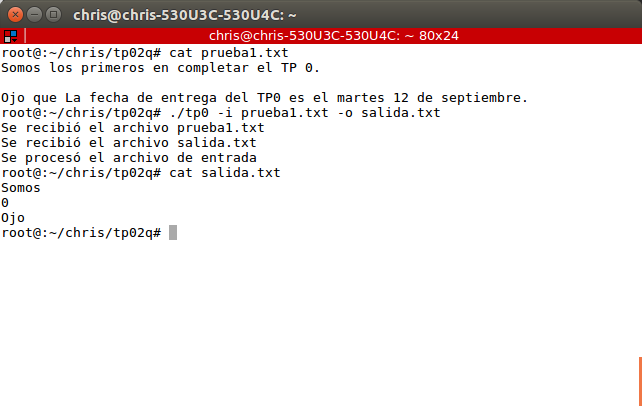
\includegraphics[width=0.5\textwidth]{prueba1.png}
\caption{Prueba utilizando archivo de entrada y salida.} \label{fig001}
\end{center}
\end{figure}

\begin{figure}[!htp]
\begin{center}
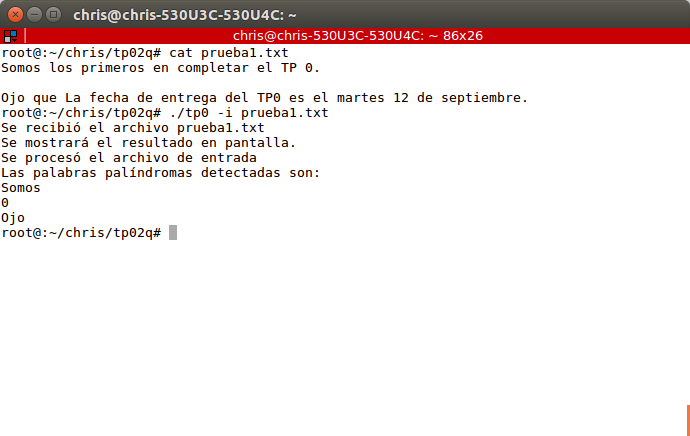
\includegraphics[width=0.5\textwidth]{prueba1SalidaPorPantalla.png}
\caption{Prueba utilizando solamente archivo de entrada.} \label{fig001}
\end{center}
\end{figure}

\begin{figure}[!htp]
\begin{center}
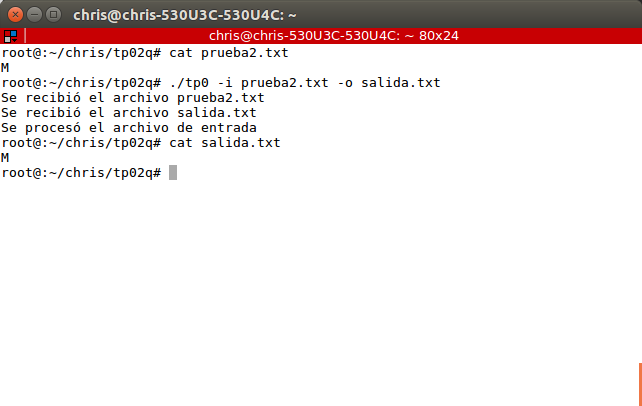
\includegraphics[width=0.5\textwidth]{prueba2.png}
\caption{Otra prueba utilizando otro archivo de entrada y salida.} \label{fig001}
\end{center}
\end{figure}

\begin{figure}[!htp]
\begin{center}
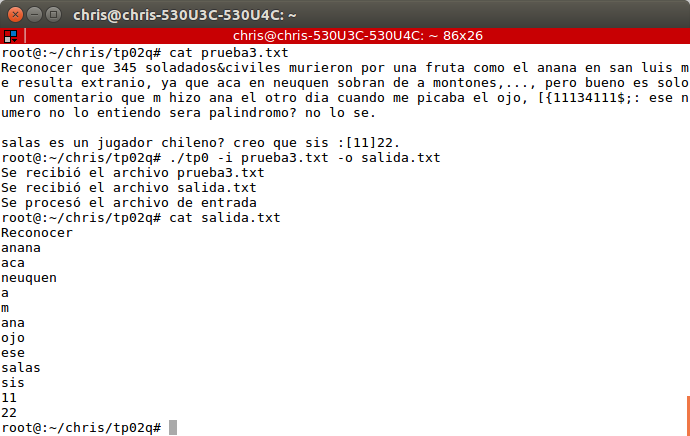
\includegraphics[width=0.5\textwidth]{prueba3.png}
\caption{Prueba utilizando otro archivo de entrada y salida.} \label{fig001}
\end{center}
\end{figure}

\begin{figure}[!htp]
\begin{center}
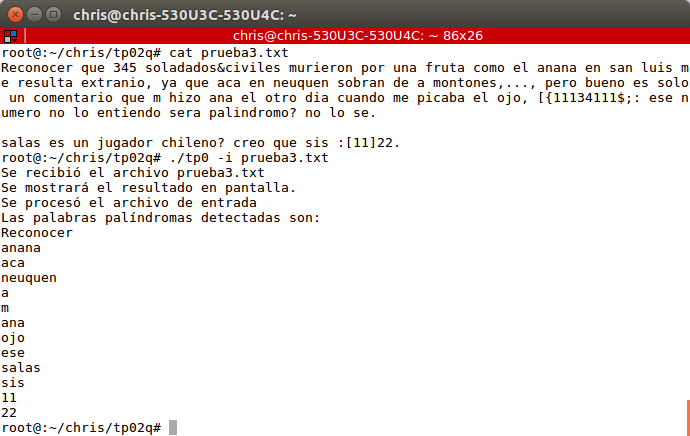
\includegraphics[width=0.5\textwidth]{prueba3salidaPorPantalla.png}
\caption{Prueba utilizando otro archivo de entrada.} \label{fig001}
\end{center}
\end{figure}

\begin{figure}[!htp]
\begin{center}
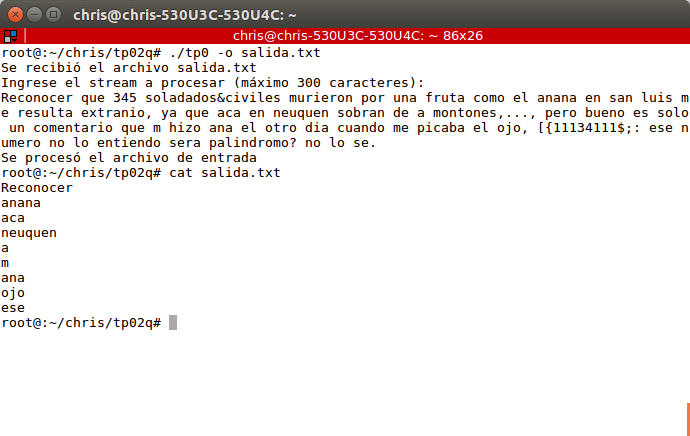
\includegraphics[width=0.5\textwidth]{pruebaPorTeclado.png}
\caption{Prueba utilizando solamente archivo de salida.} \label{fig001}
\end{center}
\end{figure}

\pagebreak
\subsection{Textos utilizados}

\paragraph{Prueba 1:}

Somos los primeros en completar el TP 0.

Ojo que La fecha de entrega del TP0 es el martes 12 de septiembre.

\paragraph{Prueba 2:}

M

\paragraph{Prueba 3:} 

Reconocer que 345 soladados&civiles murieron por una fruta como el anana en san luis me resulta extranio, ya que aca en neuquen sobran de a montones,..., pero bueno es solo un comentario que m hizo ana el otro dia cuando me picaba el ojo, [{11134111$;: ese numero no lo entiendo sera palindromo? no lo se.

salas es un jugador chileno? creo que sis :[11]22.


\section{Código MIPS generado} 

\subsection{Código fuente Assembly}
\begin{lstlisting}[language=Assembler]
    .file   1 "isPalindrome.c"
    .section .mdebug.abi32
    .previous
    .abicalls
    .text
    .align  2
    .globl  empty
    .ent    empty
empty:
    .frame  $fp,48,$ra      # vars= 8, regs= 3/0, args= 16, extra= 8
    .mask   0xd0000000,-8
    .fmask  0x00000000,0
    .set    noreorder
    .cpload $t9
    .set    reorder
    subu    $sp,$sp,48
    .cprestore 16
    sw  $ra,40($sp)
    sw  $fp,36($sp)
    sw  $gp,32($sp)
    move    $fp,$sp
    sw  $a0,48($fp)
    lw  $a0,48($fp)
    la  $t9,ftell
    jal $ra,$t9
    sw  $v0,24($fp)
    lw  $a0,48($fp)
    move    $a1,$zero
    li  $a2,2           # 0x2
    la  $t9,fseek
    jal $ra,$t9
    lw  $a0,48($fp)
    la  $t9,ftell
    jal $ra,$t9
    bne $v0,$zero,$L18
    li  $v0,1           # 0x1
    sw  $v0,28($fp)
    b   $L17
$L18:
    lw  $a0,48($fp)
    lw  $a1,24($fp)
    move    $a2,$zero
    la  $t9,fseek
    jal $ra,$t9
    sw  $zero,28($fp)
$L17:
    lw  $v0,28($fp)
    move    $sp,$fp
    lw  $ra,40($sp)
    lw  $fp,36($sp)
    addu    $sp,$sp,48
    j   $ra
    .end    empty
    .size   empty, .-empty
    .rdata
    .align  2
$LC0:
    .ascii  "El archivo %s no existe, por favor ingrese un archivo ex"
    .ascii  "istente \n\000"
    .align  2
$LC1:
    .ascii  "El archivo %s est\303\241 vac\303\255o, por favor ingres"
    .ascii  "e un archivo no vac\303\255o \n\000"
    .align  2
$LC2:
    .ascii  "Se recibi\303\263 el archivo %s \n\000"
    .text
    .align  2
    .globl  validFile
    .ent    validFile
validFile:
    .frame  $fp,48,$ra      # vars= 8, regs= 3/0, args= 16, extra= 8
    .mask   0xd0000000,-8
    .fmask  0x00000000,0
    .set    noreorder
    .cpload $t9
    .set    reorder
    subu    $sp,$sp,48
    .cprestore 16
    sw  $ra,40($sp)
    sw  $fp,36($sp)
    sw  $gp,32($sp)
    move    $fp,$sp
    sw  $a0,48($fp)
    move    $v0,$a1
    sw  $a2,56($fp)
    sb  $v0,24($fp)
    lw  $v0,48($fp)
    bne $v0,$zero,$L20
    la  $a0,$LC0
    lw  $a1,56($fp)
    la  $t9,printf
    jal $ra,$t9
    sw  $zero,28($fp)
    b   $L19
$L20:
    lw  $a0,48($fp)
    la  $t9,empty
    jal $ra,$t9
    beq $v0,$zero,$L21
    lb  $v1,24($fp)
    li  $v0,119         # 0x77
    beq $v1,$v0,$L21
    la  $a0,$LC1
    lw  $a1,56($fp)
    la  $t9,printf
    jal $ra,$t9
    sw  $zero,28($fp)
    b   $L19
$L21:
    la  $a0,$LC2
    lw  $a1,56($fp)
    la  $t9,printf
    jal $ra,$t9
    li  $v0,1           # 0x1
    sw  $v0,28($fp)
$L19:
    lw  $v0,28($fp)
    move    $sp,$fp
    lw  $ra,40($sp)
    lw  $fp,36($sp)
    addu    $sp,$sp,48
    j   $ra
    .end    validFile
    .size   validFile, .-validFile
    .align  2
    .globl  isPalindrome
    .ent    isPalindrome
isPalindrome:
    .frame  $fp,56,$ra      # vars= 16, regs= 3/0, args= 16, extra= 8
    .mask   0xd0000000,-8
    .fmask  0x00000000,0
    .set    noreorder
    .cpload $t9
    .set    reorder
    subu    $sp,$sp,56
    .cprestore 16
    sw  $ra,48($sp)
    sw  $fp,44($sp)
    sw  $gp,40($sp)
    move    $fp,$sp
    sw  $a0,56($fp)
    lw  $a0,56($fp)
    la  $t9,strlen
    jal $ra,$t9
    addu    $v0,$v0,-1
    sw  $v0,28($fp)
    sw  $zero,24($fp)
$L23:
    lw  $a0,56($fp)
    la  $t9,strlen
    jal $ra,$t9
    srl $v1,$v0,1
    lw  $v0,24($fp)
    sltu    $v0,$v0,$v1
    bne $v0,$zero,$L26
    b   $L24
$L26:
    lw  $v1,56($fp)
    lw  $v0,24($fp)
    addu    $v0,$v1,$v0
    lb  $v0,0($v0)
    sll $v1,$v0,1
    lw  $v0,_toupper_tab_
    addu    $v0,$v1,$v0
    addu    $a0,$v0,2
    lw  $v1,56($fp)
    lw  $v0,28($fp)
    addu    $v0,$v1,$v0
    lb  $v0,0($v0)
    sll $v1,$v0,1
    lw  $v0,_toupper_tab_
    addu    $v0,$v1,$v0
    addu    $v0,$v0,2
    lh  $v1,0($a0)
    lh  $v0,0($v0)
    beq $v1,$v0,$L25
    sw  $zero,32($fp)
    b   $L22
$L25:
    lw  $v0,24($fp)
    addu    $v0,$v0,1
    sw  $v0,24($fp)
    lw  $v0,28($fp)
    addu    $v0,$v0,-1
    sw  $v0,28($fp)
    b   $L23
$L24:
    li  $v0,1           # 0x1
    sw  $v0,32($fp)
$L22:
    lw  $v0,32($fp)
    move    $sp,$fp
    lw  $ra,48($sp)
    lw  $fp,44($sp)
    addu    $sp,$sp,56
    j   $ra
    .end    isPalindrome
    .size   isPalindrome, .-isPalindrome
    .rdata
    .align  2
$LC3:
    .ascii  "\n\000"
    .text
    .align  2
    .globl  seekPalindromes
    .ent    seekPalindromes
seekPalindromes:
    .frame  $fp,48,$ra      # vars= 8, regs= 3/0, args= 16, extra= 8
    .mask   0xd0000000,-8
    .fmask  0x00000000,0
    .set    noreorder
    .cpload $t9
    .set    reorder
    subu    $sp,$sp,48
    .cprestore 16
    sw  $ra,40($sp)
    sw  $fp,36($sp)
    sw  $gp,32($sp)
    move    $fp,$sp
    sw  $a0,48($fp)
    sw  $a1,52($fp)
    sw  $zero,24($fp)
$L29:
    lw  $v1,24($fp)
    move    $v0,$v1
    sll $v0,$v0,6
    addu    $v0,$v0,$v1
    sll $v1,$v0,2
    lw  $v0,48($fp)
    addu    $v0,$v1,$v0
    lb  $v1,0($v0)
    li  $v0,36          # 0x24
    bne $v1,$v0,$L31
    b   $L28
$L31:
    lw  $v1,24($fp)
    move    $v0,$v1
    sll $v0,$v0,6
    addu    $v0,$v0,$v1
    sll $v1,$v0,2
    lw  $v0,48($fp)
    addu    $v0,$v1,$v0
    move    $a0,$v0
    la  $t9,isPalindrome
    jal $ra,$t9
    beq $v0,$zero,$L32
    lw  $v1,24($fp)
    move    $v0,$v1
    sll $v0,$v0,6
    addu    $v0,$v0,$v1
    sll $v1,$v0,2
    lw  $v0,48($fp)
    addu    $v0,$v1,$v0
    move    $a0,$v0
    lw  $a1,52($fp)
    la  $t9,fputs
    jal $ra,$t9
    la  $a0,$LC3
    lw  $a1,52($fp)
    la  $t9,fputs
    jal $ra,$t9
$L32:
    lw  $v0,24($fp)
    addu    $v0,$v0,1
    sw  $v0,24($fp)
    b   $L29
$L28:
    move    $sp,$fp
    lw  $ra,40($sp)
    lw  $fp,36($sp)
    addu    $sp,$sp,48
    j   $ra
    .end    seekPalindromes
    .size   seekPalindromes, .-seekPalindromes
    .rdata
    .align  2
$LC4:
    .ascii  "Las palabras pal\303\255ndromas detectadas son: \n\000"
    .align  2
$LC5:
    .ascii  "%s\000"
    .text
    .align  2
    .globl  printPalindromes
    .ent    printPalindromes
printPalindromes:
    .frame  $fp,304,$ra     # vars= 264, regs= 3/0, args= 16, extra= 8
    .mask   0xd0000000,-8
    .fmask  0x00000000,0
    .set    noreorder
    .cpload $t9
    .set    reorder
    subu    $sp,$sp,304
    .cprestore 16
    sw  $ra,296($sp)
    sw  $fp,292($sp)
    sw  $gp,288($sp)
    move    $fp,$sp
    sw  $a0,304($fp)
    addu    $a0,$fp,24
    move    $a1,$zero
    li  $a2,260         # 0x104
    la  $t9,memset
    jal $ra,$t9
    lw  $a0,304($fp)
    la  $t9,rewind
    jal $ra,$t9
    addu    $a0,$fp,24
    li  $a1,260         # 0x104
    lw  $a2,304($fp)
    la  $t9,fgets
    jal $ra,$t9
    la  $a0,$LC4
    la  $t9,printf
    jal $ra,$t9
$L34:
    lw  $v0,304($fp)
    lhu $v0,12($v0)
    srl $v0,$v0,5
    andi    $v0,$v0,0x1
    beq $v0,$zero,$L36
    b   $L33
$L36:
    la  $a0,$LC5
    addu    $a1,$fp,24
    la  $t9,printf
    jal $ra,$t9
    addu    $a0,$fp,24
    move    $a1,$zero
    li  $a2,260         # 0x104
    la  $t9,memset
    jal $ra,$t9
    addu    $a0,$fp,24
    li  $a1,260         # 0x104
    lw  $a2,304($fp)
    la  $t9,fgets
    jal $ra,$t9
    b   $L34
$L33:
    move    $sp,$fp
    lw  $ra,296($sp)
    lw  $fp,292($sp)
    addu    $sp,$sp,304
    j   $ra
    .end    printPalindromes
    .size   printPalindromes, .-printPalindromes
    .align  2
    .globl  validCharacter
    .ent    validCharacter
validCharacter:
    .frame  $fp,32,$ra      # vars= 16, regs= 2/0, args= 0, extra= 8
    .mask   0x50000000,-4
    .fmask  0x00000000,0
    .set    noreorder
    .cpload $t9
    .set    reorder
    subu    $sp,$sp,32
    .cprestore 0
    sw  $fp,28($sp)
    sw  $gp,24($sp)
    move    $fp,$sp
    move    $v0,$a0
    sb  $v0,8($fp)
    lb  $v0,8($fp)
    sw  $v0,12($fp)
    lw  $v0,12($fp)
    slt $v0,$v0,58
    beq $v0,$zero,$L38
    lw  $v0,12($fp)
    slt $v0,$v0,48
    bne $v0,$zero,$L38
    li  $v0,1           # 0x1
    sw  $v0,16($fp)
    b   $L37
$L38:
    lw  $v0,12($fp)
    slt $v0,$v0,91
    beq $v0,$zero,$L39
    lw  $v0,12($fp)
    slt $v0,$v0,65
    bne $v0,$zero,$L39
    li  $v0,1           # 0x1
    sw  $v0,16($fp)
    b   $L37
$L39:
    lw  $v0,12($fp)
    slt $v0,$v0,123
    beq $v0,$zero,$L40
    lw  $v0,12($fp)
    slt $v0,$v0,97
    bne $v0,$zero,$L40
    li  $v0,1           # 0x1
    sw  $v0,16($fp)
    b   $L37
$L40:
    lw  $v1,12($fp)
    li  $v0,45          # 0x2d
    bne $v1,$v0,$L41
    li  $v0,1           # 0x1
    sw  $v0,16($fp)
    b   $L37
$L41:
    lw  $v1,12($fp)
    li  $v0,95          # 0x5f
    bne $v1,$v0,$L42
    li  $v0,1           # 0x1
    sw  $v0,16($fp)
    b   $L37
$L42:
    sw  $zero,16($fp)
$L37:
    lw  $v0,16($fp)
    move    $sp,$fp
    lw  $fp,28($sp)
    addu    $sp,$sp,32
    j   $ra
    .end    validCharacter
    .size   validCharacter, .-validCharacter
    .align  2
    .globl  parseLine
    .ent    parseLine
parseLine:
    .frame  $fp,56,$ra      # vars= 16, regs= 3/0, args= 16, extra= 8
    .mask   0xd0000000,-8
    .fmask  0x00000000,0
    .set    noreorder
    .cpload $t9
    .set    reorder
    subu    $sp,$sp,56
    .cprestore 16
    sw  $ra,48($sp)
    sw  $fp,44($sp)
    sw  $gp,40($sp)
    move    $fp,$sp
    sw  $a0,56($fp)
    sw  $a1,60($fp)
    sb  $zero,24($fp)
    sw  $zero,28($fp)
    sw  $zero,32($fp)
    sw  $zero,36($fp)
$L44:
    lbu $v0,24($fp)
    beq $v0,$zero,$L46
    b   $L45
$L46:
    lw  $v1,56($fp)
    lw  $v0,28($fp)
    addu    $v0,$v1,$v0
    lb  $v0,0($v0)
    move    $a0,$v0
    la  $t9,validCharacter
    jal $ra,$t9
    beq $v0,$zero,$L47
    lw  $v1,32($fp)
    move    $v0,$v1
    sll $v0,$v0,6
    addu    $v0,$v0,$v1
    sll $v1,$v0,2
    lw  $v0,60($fp)
    addu    $v1,$v1,$v0
    lw  $v0,36($fp)
    addu    $a0,$v1,$v0
    lw  $v1,56($fp)
    lw  $v0,28($fp)
    addu    $v0,$v1,$v0
    lbu $v0,0($v0)
    sb  $v0,0($a0)
    lw  $v0,36($fp)
    addu    $v0,$v0,1
    sw  $v0,36($fp)
    b   $L48
$L47:
    lw  $v0,36($fp)
    beq $v0,$zero,$L48
    lw  $v1,32($fp)
    move    $v0,$v1
    sll $v0,$v0,6
    addu    $v0,$v0,$v1
    sll $v1,$v0,2
    lw  $v0,60($fp)
    addu    $v1,$v1,$v0
    lw  $v0,36($fp)
    addu    $v0,$v1,$v0
    sb  $zero,0($v0)
    sw  $zero,36($fp)
    lw  $v0,32($fp)
    addu    $v0,$v0,1
    sw  $v0,32($fp)
$L48:
    lw  $v1,56($fp)
    lw  $v0,28($fp)
    addu    $v0,$v1,$v0
    lb  $v1,0($v0)
    li  $v0,10          # 0xa
    beq $v1,$v0,$L51
    lw  $v1,56($fp)
    lw  $v0,28($fp)
    addu    $v0,$v1,$v0
    lb  $v0,0($v0)
    bne $v0,$zero,$L50
$L51:
    li  $v0,1           # 0x1
    sb  $v0,24($fp)
$L50:
    lw  $v0,28($fp)
    addu    $v0,$v0,1
    sw  $v0,28($fp)
    b   $L44
$L45:
    lw  $v1,32($fp)
    move    $v0,$v1
    sll $v0,$v0,6
    addu    $v0,$v0,$v1
    sll $v1,$v0,2
    lw  $v0,60($fp)
    addu    $v1,$v1,$v0
    li  $v0,36          # 0x24
    sb  $v0,0($v1)
    move    $sp,$fp
    lw  $ra,48($sp)
    lw  $fp,44($sp)
    addu    $sp,$sp,56
    j   $ra
    .end    parseLine
    .size   parseLine, .-parseLine
    .rdata
    .align  2
$LC6:
    .ascii  "Se proces\303\263 el archivo de entrada \n\000"
    .text
    .align  2
    .globl  processInput
    .ent    processInput
processInput:
    .frame  $fp,67912,$ra       # vars= 67872, regs= 3/0, args= 16, extra= 8
    .mask   0xd0000000,-8
    .fmask  0x00000000,0
    .set    noreorder
    .cpload $t9
    .set    reorder
    subu    $sp,$sp,67912
    .cprestore 16
    li  $t5,65536           # 0x10000
    ori $t5,$t5,0x940
    addu    $t5,$t5,$sp
    sw  $ra,0($t5)
    sw  $fp,-4($t5)
    sw  $gp,-8($t5)
    move    $fp,$sp
    sw  $a0,67912($fp)
    sw  $a1,67916($fp)
    move    $v0,$a2
    sb  $v0,24($fp)
    lw  $a0,67912($fp)
    la  $t9,rewind
    jal $ra,$t9
    addu    $v0,$fp,32
    move    $a0,$v0
    li  $a1,260         # 0x104
    lw  $a2,67912($fp)
    la  $t9,fgets
    jal $ra,$t9
$L53:
    lw  $v0,67912($fp)
    lhu $v0,12($v0)
    srl $v0,$v0,5
    andi    $v0,$v0,0x1
    beq $v0,$zero,$L55
    b   $L54
$L55:
    addu    $v0,$fp,32
    addu    $v1,$fp,296
    move    $a0,$v0
    move    $a1,$v1
    la  $t9,parseLine
    jal $ra,$t9
    addu    $v0,$fp,296
    move    $a0,$v0
    lw  $a1,67916($fp)
    la  $t9,seekPalindromes
    jal $ra,$t9
    addu    $v0,$fp,32
    move    $a0,$v0
    li  $a1,260         # 0x104
    lw  $a2,67912($fp)
    la  $t9,fgets
    jal $ra,$t9
    b   $L53
$L54:
    lw  $a0,67912($fp)
    la  $t9,fclose
    jal $ra,$t9
    la  $a0,$LC6
    la  $t9,printf
    jal $ra,$t9
    lbu $v0,24($fp)
    beq $v0,$zero,$L56
    lw  $a0,67916($fp)
    la  $t9,printPalindromes
    jal $ra,$t9
$L56:
    lw  $a0,67916($fp)
    la  $t9,fclose
    jal $ra,$t9
    li  $t4,65536           # 0x10000
    ori $t4,$t4,0x948
    move    $sp,$fp
    addu    $t5,$t4,$sp
    lw  $ra,-8($t5)
    lw  $fp,-12($t5)
    addu    $sp,$sp,$t4
    j   $ra
    .end    processInput
    .size   processInput, .-processInput
    .rdata
    .align  2
$LC8:
    .ascii  "version\000"
    .align  2
$LC9:
    .ascii  "help\000"
    .align  2
$LC10:
    .ascii  "input\000"
    .align  2
$LC11:
    .ascii  "output\000"
    .data
    .align  2
$LC12:
    .word   $LC8
    .word   0
    .word   0
    .word   86
    .word   $LC9
    .word   0
    .word   0
    .word   104
    .word   $LC10
    .word   1
    .word   0
    .word   105
    .word   $LC11
    .word   1
    .word   0
    .word   111
    .word   0
    .word   0
    .word   0
    .word   0
    .globl  memcpy
    .rdata
    .align  2
$LC7:
    .ascii  "i:o:hV\000"
    .align  2
$LC13:
    .ascii  "inputFileAux.txt\000"
    .align  2
$LC14:
    .ascii  "outputFileAux.txt\000"
    .align  2
$LC15:
    .ascii  "Debe ingresar alg\303\272n argumento, para mas informaci"
    .ascii  "\303\263n ingrese -h \n\000"
    .align  2
$LC16:
    .ascii  "TP #0 de la materia Organizaci\303\263n de Computadoras "
    .ascii  "\n\000"
    .align  2
$LC17:
    .ascii  "Alumnos: \n\000"
    .align  2
$LC18:
    .ascii  "\tFl\303\263rez Del Carpio Christian\n"
    .ascii  "\tMontenegro Josefina \n"
    .ascii  "\tQuino Lopez Julian \n\000"
    .align  2
$LC19:
    .ascii  "Usage: \n\000"
    .align  2
$LC20:
    .ascii  "\t%s -h \n\000"
    .align  2
$LC21:
    .ascii  "\t%s -V \n\000"
    .align  2
$LC22:
    .ascii  "\t%s [options] \n\000"
    .align  2
$LC23:
    .ascii  "Options: \n\000"
    .align  2
$LC24:
    .ascii  "\t-V, --version  Print version and quit. \n\000"
    .align  2
$LC25:
    .ascii  "\t-h, --help     Print this information. \n\000"
    .align  2
$LC26:
    .ascii  "\t-o, --output   Location of the output file. \n\000"
    .align  2
$LC27:
    .ascii  "\t-i, --input    Location of the input file. \n\000"
    .align  2
$LC28:
    .ascii  "r\000"
    .align  2
$LC29:
    .ascii  "w\000"
    .align  2
$LC30:
    .ascii  "Opci\303\263n inv\303\241lida. Para ver m\303\241s infor"
    .ascii  "maci\303\263n ingrese -h. \n\000"
    .align  2
$LC31:
    .ascii  "Ingrese el stream a procesar (m\303\241ximo 300 caracter"
    .ascii  "es): \n\000"
    .align  2
$LC32:
    .ascii  "w+\000"
    .align  2
$LC33:
    .ascii  "Se mostrar\303\241 el resultado en pantalla. \n\000"
    .text
    .align  2
    .globl  main
    .ent    main
main:
    .frame  $fp,472,$ra     # vars= 424, regs= 3/0, args= 24, extra= 8
    .mask   0xd0000000,-8
    .fmask  0x00000000,0
    .set    noreorder
    .cpload $t9
    .set    reorder
    subu    $sp,$sp,472
    .cprestore 24
    sw  $ra,464($sp)
    sw  $fp,460($sp)
    sw  $gp,456($sp)
    move    $fp,$sp
    sw  $a0,472($fp)
    sw  $a1,476($fp)
    sw  $zero,32($fp)
    la  $v0,$LC7
    sw  $v0,36($fp)
    addu    $v0,$fp,40
    la  $v1,$LC12
    move    $a0,$v0
    move    $a1,$v1
    li  $a2,80          # 0x50
    la  $t9,memcpy
    jal $ra,$t9
    sw  $zero,120($fp)
    sw  $zero,124($fp)
    sb  $zero,128($fp)
    sb  $zero,129($fp)
    la  $v0,$LC13
    sw  $v0,440($fp)
    la  $v0,$LC14
    sw  $v0,444($fp)
    lw  $v1,472($fp)
    li  $v0,1           # 0x1
    bne $v1,$v0,$L58
    la  $a0,$LC15
    la  $t9,printf
    jal $ra,$t9
    sw  $zero,448($fp)
    b   $L57
$L58:
    .set    noreorder
    nop
    .set    reorder
$L59:
    addu    $v0,$fp,40
    sw  $zero,16($sp)
    lw  $a0,472($fp)
    lw  $a1,476($fp)
    lw  $a2,36($fp)
    move    $a3,$v0
    la  $t9,getopt_long
    jal $ra,$t9
    sw  $v0,32($fp)
    lw  $v1,32($fp)
    li  $v0,-1          # 0xffffffffffffffff
    bne $v1,$v0,$L61
    b   $L60
$L61:
    lw  $v0,32($fp)
    sw  $v0,452($fp)
    li  $v0,104         # 0x68
    lw  $v1,452($fp)
    beq $v1,$v0,$L64
    lw  $v1,452($fp)
    slt $v0,$v1,105
    beq $v0,$zero,$L71
    li  $v0,86          # 0x56
    lw  $v1,452($fp)
    beq $v1,$v0,$L63
    b   $L69
$L71:
    li  $v0,105         # 0x69
    lw  $v1,452($fp)
    beq $v1,$v0,$L65
    li  $v0,111         # 0x6f
    lw  $v1,452($fp)
    beq $v1,$v0,$L67
    b   $L69
$L63:
    la  $a0,$LC16
    la  $t9,printf
    jal $ra,$t9
    la  $a0,$LC17
    la  $t9,printf
    jal $ra,$t9
    la  $a0,$LC18
    la  $t9,printf
    jal $ra,$t9
    sw  $zero,448($fp)
    b   $L57
$L64:
    la  $a0,$LC19
    la  $t9,printf
    jal $ra,$t9
    lw  $v0,476($fp)
    la  $a0,$LC20
    lw  $a1,0($v0)
    la  $t9,printf
    jal $ra,$t9
    lw  $v0,476($fp)
    la  $a0,$LC21
    lw  $a1,0($v0)
    la  $t9,printf
    jal $ra,$t9
    lw  $v0,476($fp)
    la  $a0,$LC22
    lw  $a1,0($v0)
    la  $t9,printf
    jal $ra,$t9
    la  $a0,$LC23
    la  $t9,printf
    jal $ra,$t9
    la  $a0,$LC24
    la  $t9,printf
    jal $ra,$t9
    la  $a0,$LC25
    la  $t9,printf
    jal $ra,$t9
    la  $a0,$LC26
    la  $t9,printf
    jal $ra,$t9
    la  $a0,$LC27
    la  $t9,printf
    jal $ra,$t9
    sw  $zero,448($fp)
    b   $L57
$L65:
    lw  $a0,optarg
    la  $a1,$LC28
    la  $t9,fopen
    jal $ra,$t9
    sw  $v0,120($fp)
    lw  $a0,120($fp)
    li  $a1,114         # 0x72
    lw  $a2,optarg
    la  $t9,validFile
    jal $ra,$t9
    bne $v0,$zero,$L59
    sw  $zero,448($fp)
    b   $L57
$L67:
    lw  $a0,optarg
    la  $a1,$LC29
    la  $t9,fopen
    jal $ra,$t9
    sw  $v0,124($fp)
    lw  $a0,124($fp)
    li  $a1,119         # 0x77
    lw  $a2,optarg
    la  $t9,validFile
    jal $ra,$t9
    bne $v0,$zero,$L59
    sw  $zero,448($fp)
    b   $L57
$L69:
    la  $a0,$LC30
    la  $t9,printf
    jal $ra,$t9
    b   $L59
$L60:
    lw  $v0,120($fp)
    bne $v0,$zero,$L72
    la  $a0,$LC31
    la  $t9,printf
    jal $ra,$t9
    addu    $v0,$fp,136
    move    $a0,$v0
    li  $a1,300         # 0x12c
    la  $a2,__sF
    la  $t9,fgets
    jal $ra,$t9
    lw  $a0,440($fp)
    la  $a1,$LC32
    la  $t9,fopen
    jal $ra,$t9
    sw  $v0,120($fp)
    addu    $v0,$fp,136
    move    $a0,$v0
    lw  $a1,120($fp)
    la  $t9,fputs
    jal $ra,$t9
    la  $a0,$LC3
    lw  $a1,120($fp)
    la  $t9,fputs
    jal $ra,$t9
    li  $v0,1           # 0x1
    sb  $v0,128($fp)
$L72:
    lw  $v0,124($fp)
    bne $v0,$zero,$L73
    la  $a0,$LC33
    la  $t9,printf
    jal $ra,$t9
    lw  $a0,444($fp)
    la  $a1,$LC32
    la  $t9,fopen
    jal $ra,$t9
    sw  $v0,124($fp)
    li  $v0,1           # 0x1
    sb  $v0,129($fp)
$L73:
    lbu $v0,129($fp)
    lw  $a0,120($fp)
    lw  $a1,124($fp)
    move    $a2,$v0
    la  $t9,processInput
    jal $ra,$t9
    lbu $v0,128($fp)
    beq $v0,$zero,$L74
    lw  $a0,440($fp)
    la  $t9,remove
    jal $ra,$t9
$L74:
    lbu $v0,129($fp)
    beq $v0,$zero,$L75
    lw  $a0,444($fp)
    la  $t9,remove
    jal $ra,$t9
$L75:
    sw  $zero,448($fp)
$L57:
    lw  $v0,448($fp)
    move    $sp,$fp
    lw  $ra,464($sp)
    lw  $fp,460($sp)
    addu    $sp,$sp,472
    j   $ra
    .end    main
    .size   main, .-main
    .ident  "GCC: (GNU) 3.3.3 (NetBSD nb3 20040520)"

\end{lstlisting}


\section{Conclusiones}

El trabajo práctico nos resultó interesante, no por el programa a desarrollar en sí, sino por lo que representó trabajar con el emulador GXEmul, emular la arquitectura MIPS, crear el túnel de comunicación entre el host OS (Linux, distribución Ubuntu) y el guest OS (NetBSD). Aprendimos como transferir archivos entre ambos sistemas y también ciertas cuestiones del lenguaje C con el cual no estábamos toalmente familiarizados.

\begin{thebibliography}{1}

\bibitem{lib} GetOpt library, https://www.gnu.org/software/libc/manual/html_node/Example-of-Getopt.html.

\bibitem{stack} StackOverflow, https://www.stackoverflow.com.

\end{thebibliography}

\end{document}
